\chapter{Background}
%https://www.researchgate.net/figure/A-bidirectional-system-with-distributed-generation_fig2_286569839
%This section gives an overview of the conducted research work to provide a central theme for the reader of this doctoral thesis. This overview should help to understand each individual paper in the annex, representing essential parts of this doctoral thesis, in the overall context of the developed optimization methodology.

The voltage control problem has been studied for years, but it only comes under the spotlight in recent years for the increasing number of distributed resources introduced in the networks. It is important to control the voltage in an electrical power system for a regular operation of the electrical equipment, to prevent damage such as overheating of generators and motors, to reduce transmission losses and to maintain the ability of the system to last and prevent voltage collapse. \\

%https://electrical-engineering-portal.com/how-reactive-power-is-helpful-to-maintain-a-system-healthy
In particular, it is useful and needed to reduce the output of renewable generators from what they could otherwise have produced given the available resources, often referred to as the process of \textbf{curtailment}. Such generation curtailment, along with storage and transmission losses, constitute the principal sources of energy loss that could be minimised with active network management \gls{ANM} \cite{gym-anm}. \\

\noindent Controlling the voltage in an active way has many interesting properties:
\begin{itemize}
    \item It is a combination of local and global problem: the voltage at each node is influenced by the powers of all other nodes, but the impact depends on the distance between them.
    \item It is a constrained optimization problem where the constraint is to keep the voltage in a given range and the objective is to minimise the total power loss.
    \item Voltage control has a relatively large tolerance, and there are no severe consequences if the control fails to meet the requirements for short periods of time. \cite{wang2022multiagent}
    \item It is a hierarchical problem where much information is available at the top of the pyramid (distribution stations and substations) and they decrease at the base of the pyramid (houses, factories) mainly due to the absence of many sensors.
\end{itemize}

\section{Power system}
\subsection{Description of a power system}
%https://www.generatorsource.com/Articles/Generator-Info/High-Medium-and-Low-Voltage-Differences.aspx
%Power systems are facilities that produce and transport electricity to consumers. \\
Power transmission systems consist of an interconnected set of overhead lines, cables and related equipment that are used for the transfer of electricity at high voltage levels
between supply points and load points, such as customers and other electric systems. \\

In the traditional power system, electricity is produced in large, centralised power plants. The electricity is then transferred to the loads using the transmission and distribution networks. High and extra-high voltages are associated with supply transmission from the power plant. The reason for transmitting power at high and extra-high voltage levels is to increase efficiency. The lower current accompanying the high voltage transmission allows for the use of thinner, lighter-weight cables. This reduces the cost in the tower and electrical line construction. In Belgium, High and extra-high voltages refer to voltage magnitudes $30 kV \leq V < 380 kV$ for the high voltage and $V \geq 380 kV$ for the extra high voltage \cite{elia}. (\emph{Symbols problem: V for voltage magnitude and V for volts?})\\
Large industrial complexes and factories that require a substantial amount of power often utilise medium supply voltages. The high voltage coming from the power plant is sent to the primary substation, this can supply step-down power to secondary substations or to single buildings. Secondary substations can have transformers to further step down the power, and they are generally located in areas that can serve one or more buildings. Medium voltages refer to voltage magnitude $0.4 kV \leq V < 30 kV$. \\
Then the medium supply power is step down again to a low voltage and sent to the domestic household or home appliances power supply. Low voltages refer to voltage magnitude $V < 0.4 kV$. \\
\begin{figure}[H]
\centering
    % 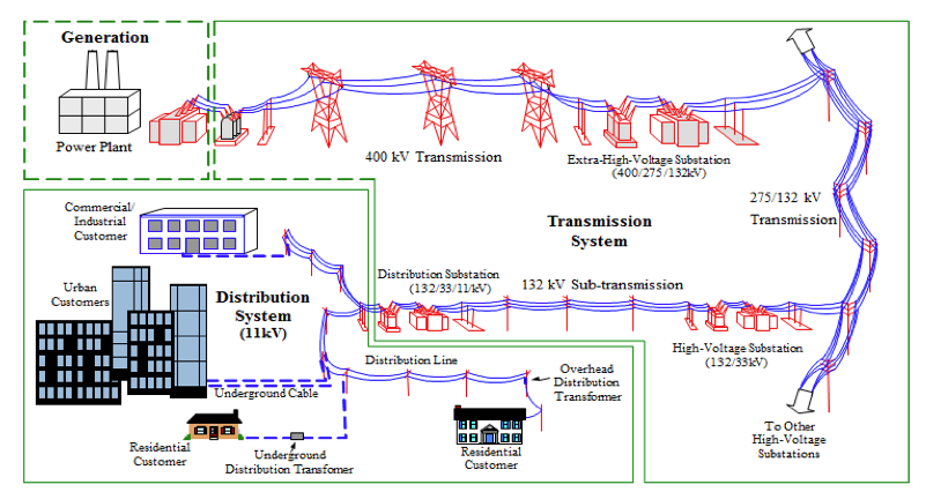
\includegraphics[width=.9\linewidth]{images/DN/HighMediumLowV.png}
    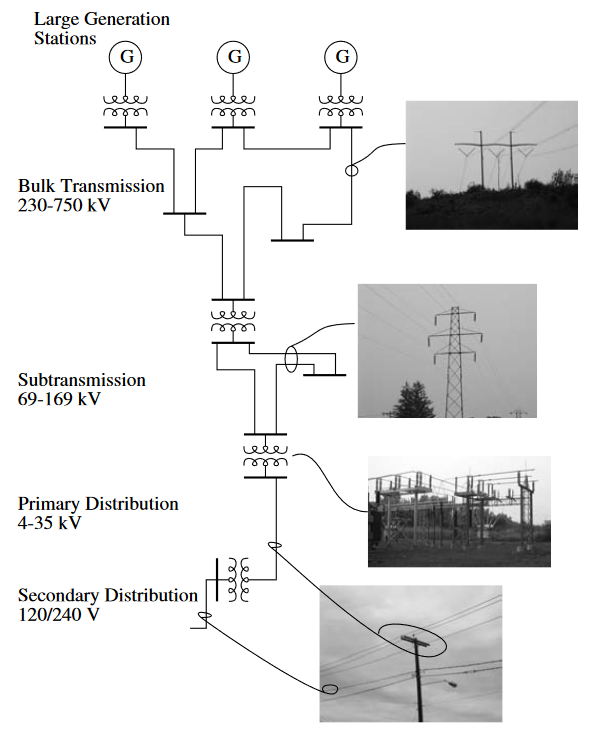
\includegraphics[width=.25\linewidth]{images/Background/DN/DN.PNG}
\caption[Power network distribution]{Power network distribution \cite{EPD}}
% \label{fig:gym_anm_net}
\end{figure}


\noindent A power system is usually made up of the following main elements: \label{networkeledesc}
\begin{itemize}
    \item \textbf{Generator}. These produce energy, converting a form of energy into electricity. Many generators produce energy using turbines: a mass of air or water spin the generator's blades, producing electricity. This mass can be natural: hydroelectric, wind or geothermal turbines, or generated by combustion of some fuel, for example natural gas or nuclear source. \\
    There are other generators that do not need a turbine to generate electricity, for example solar panels.
    \item \textbf{Transformers}. Transformers are used to interlink systems operating at different voltages. These can increase  the voltage magnitude near a generator power plant or decrease it near the consumptions facilities. \\
    Changing the voltage magnitude allows reducing the power loss due to transportation: the power lost is given by $P=VI$, where \gls{V} is the voltage and \gls{I} is the current, so decreasing the voltage can reduce the energy loss.
    \item \textbf{Lines}. These transport the power from where energy is generated to where it is consumed. One of the main issues about transportation lines is insulation. \\
    There are different types of lines: overhead cables, they use air to insulate the bare conductors or underground cables, for these cables particular attention must be taken to insulate them from other conductors and from the earth (ground). Also, the material used must be resistant to damages, corrosion, and it must avoid that the water is being absorbed.
    \item \textbf{Switchgear}. In an electricity supply, it is necessary to disconnect equipment from the network quickly if a fault occurs to avoid damage on the elements of the network, or to disconnect some points of the network to avoid excessive losses or too high or low voltages. \\
    Switchgear is a broad term that describes a wide variety of switching devices that fulfil the need of controlling, protecting, and isolating power systems. Among these switching devices the most common are: \emph{circuit breaker}, during an electrical fault, a circuit breaker will detect the anomaly and interrupt the power flow, effectively limiting damage to the system; \emph{switch} is an electrical component that can disconnect or connect the conducting path in an electrical circuit, interrupting the electric current or diverting it from one conductor to another; \emph{recloser} similar to the circuit breaker but used in high voltage networks, these devices handle trouble temporary occurrences such as lightning, windblown tree branches or wires,
    birds, or rodents damaging the wires.
    
    \item \textbf{Loads} are electric components that consume the electric power generated by the generators. The type of loads can be divided base on the consumption in:
    \begin{itemize}
        \item[] \emph{Domestic loads}, the domestic loads mainly consist of lights, fan, refrigerator, air conditioners, mixer, grinder, heater, ovens, small pumping, motor, etc. The domestic loads consume very little power.
        \item[] \emph{Commercial loads}, the commercial loads mainly consist of lightning, fans, heating, air conditioning and many other electrical appliances used in establishments such as markets, restaurants, shops. This type of load occurs for more hours during the day as compared to the domestic load.
        \item[] \emph{Industrial loads}, the domestic loads refer from a small-scale industry, to a heavy industry. It includes all electrical loads used in industries along with the employed machinery. Industrial loads may be connected during the whole day \cite{EDNdesign}.
    \end{itemize}
    % \item Load buses where \gls{P} and \gls{Q} are specified.
    % \item Generator buses where the voltage magnitude \gls{V} and the power \gls{P} are specified.
    % \item A primary bus, an "infinite" bus, where the magnitude voltage \gls{V} is specified (normally 1 \gls{pu}) and its phase angle \gls{Vangle} is assumed to be zero as a reference angle. At this bus, both \gls{P} and \gls{Q} can be what is needed to keep the network stable. \cite{eps}
\end{itemize}

\subsection{Power flow}
\label{powerflow}
%Mathmatical formulation: https://www.engineering.iastate.edu/~jdm/ee458_2011/PowerFlowEquations.pdf
%Simple discussion: https://www.pterra.com/power-flow-analysis/power-flow-solution-techniques/
An important procedure in power system networks is to perform a numerical analysis to determine the electrical state of the network, starting from some parameters that are known. This analysis is called optimal power flow (\gls{OPF}).\\
The \gls{OPF} is an optimization problem essential for planning purposes: besides the calculation of electrical characteristics of the power system, power flow analysis can also help to optimize the system operating conditions, minimize the power losses and determine control actions to satisfy the demand while meeting operational constraints.

\subsubsection{Buses}
The power flow gives information about the steady state of the entire system such as voltage, real and reactive power, line loadings and power injection.\\
Each bus is associated with four quantities: voltage magnitude \gls{V}, phase angle \gls{angleV}, real power \gls{AP} and reactive power \gls{Q}.
Depending on the quantity that have been specified, buses in the power system are classified into the following three different types:
\begin{itemize}
    \item \textbf{Slack bus}. It is taken as reference where the magnitude and phase angle of the voltage are specified. Slack bus magnitude considers 1 \gls{pu} and phase angle 0 degrees. This bus provides the additional real and reactive power to supply the transmission losses, since there are unknown until the final solution is obtained.

    \item \textbf{Load buses or PQ bus}. At these buses, the real and reactive powers are specified. The magnitude and phase angle of the bus voltage are unknown until the final solution is obtained.

    \item \textbf{Voltage controlled buses or PV bus}. At these buses, the real power and voltage magnitude are specified. The phase angles of the voltages and the reactive power are unknown until the final solution is obtained. The limits on the value of reactive power are also specified. 
\end{itemize}

\subsubsection{Solution techniques}
Defining and solving the power flow equations are the main tasks in load flow analysis. \\
The definition of the power flow equations is based on Ohm’s Law, which is the relationship between voltages and currents. For a network, it can be expressed in matrix notation as follows:
\[
    \mathbf{Y} \times \mathbf{V} = \mathbf{I}
\]
\[
 \begin{bmatrix}
 Y_{1,1} & \quad & \cdots & \quad & Y_{1,N} \\
 &  &  \\
 Y_{2,1} & \quad & \cdots & \quad & Y_{2,N} \\
 &  &  \\
 \vdots & \quad & \ddots & \quad & \vdots \\
 &  &  \\
 Y_{N,1} & \quad & \cdots & \quad & Y_{N,N} \\
 \end{bmatrix}
 \times
 \begin{bmatrix}
 V_1 \\ \\ V_2 \\ \\ \vdots \\ \\ V_N
 \end{bmatrix}
 =
 \begin{bmatrix}
 I_1 \\  \\ I_2 \\ \\ \vdots \\  \\ I_N
 \end{bmatrix}
\]

\noindent Where:
\begin{itemize}
    \item \textbf{Y} is the bus admittance matrix
    \item \textbf{V} is an array of bus voltages
    \item \textbf{I} is an array of bus current injections (positive value when generation, and negative value when load)
\end{itemize}

The power flow formulation is based on the application of Kirchhoff’s laws to meshed electric networks. The basic concept is that the sum of all flows into each and every node should be equal to zero.\\
The flows are in complex form, they consist of real and reactive components, or \glspl{W} and \glspl{VAR}. If there are n nodes, then there are n complex equations. The resulting system of equations involves non-linear relationships, making the calculations not easy. Solution methods are primarily iterative with the objective of reducing the sum of flows in all nodes to some acceptably small value known as the mismatch tolerance. \\

All these iterative methods follow the same basic concept: they assume starting values for the dependent variables, primarily voltage at nominal voltage magnitude (i.e. 1 \gls{pu}) and zero phase angle; compute new values for those voltages using the nodal network equation or a numerical approximation and repeat until the convergence criteria are met. \\

The solution has to satisfy some network constrains, in particular:
\begin{itemize}
    \item Active and reactive power balance: the sum of the power injections (that can be positive or negative) at each bus must be equal to 0. This, as said, results from the Kirchhoff’s laws.
    
    \item Voltage limits: the voltage magnitude at each bus and the voltage phase difference between two directly connected buses are bounded by some specific values to maintain safe operation.
    
    \item Thermal limits on transmission lines: the flow in each transmission line is limited due to the thermal limit of the conductors.
    
    \item Generator active and reactive power limits: the generating units have    generally a minimum and maximum level of output power.
    
    \item Generator ramping limits: the output power of a generating unit can not be instantaneously increased or decreased. The operator must take into account the ramping limits of the generators.
\end{itemize}

\subsubsection{Convergence}
The \gls{OPF} is a non-linear and non-convex optimization problem, with a large number of constraints (both equality and inequality constraints) and variables (that can be both continuous and discrete). It is therefore a hard problem, whose solution cost increase exponentially, particularly with the increasing size of the network. Moreover, there is no guarantee to find the global optimum. \\
When a solution exists and it is reached, it is said that the network has converged. Convergence is the state when all nodes have met the mismatch tolerance. The main power flow solution methods are:
\begin{itemize}
    \item Gauss-Seidel method updates the voltage one node at a time until all nodes are within the mismatch tolerance.
    
    \item Newton-Raphson method uses a first order expansion of the power flow equations to approach convergence. Generally faster than the Gauss-Seidel method and able to converge to small tolerances. However, the method is prone to the phenomenon of \textbf{divergence}, when mismatches increase instead of decrease from iteration to iteration. This occurs when the solution vector exits outside the feasible solution space at any point during the algorithm. Once outside feasible space, the solution gradient tends to further increase mismatches, leading to solutions that “blow-up” in the numerical sense. This method requires calculating the first order approximation matrix (known as the Jacobian). \\
    Several variations on the Newton-Raphson are in use, including:
        \begin{itemize}
            \item[] Fast Decoupled: separates the loosely linked real and reactive components of the power flow equations in order to speed up solution.
            \item[] Fixed Newton: does not update the first order approximation matrix every iteration to reduce computational burden.
            \item[] Non-divergent power flow: applies a reduction to the Jacobian multiplier whenever the solution appears to exit feasible space. In certain situations, this may prevent divergence, or at least stop it before blow-up.
        \end{itemize}
    \item Interior-Point Newton method forces the solution inside feasible space to avoid divergence. The interior point method uses a second order expansion of the power flow equations as a basis for its algorithm. The method is more computationally intensive than either the Gauss-Seidel or Newton-Raphson, but is less susceptible to numerical divergence.
\end{itemize}

\subsubsection{Divergence}
Divergence is the condition of the power network when the numerical solution can not be found any more due to some possible issues:

\begin{itemize}
    \item the power system is going to “blow-up.”
    \item the power system is in voltage collapse.
    \item the power system is unstable.
    \item the initial conditions defined were bad or poor.
    \item some issues related to software or input data.
\end{itemize}

Divergence of the power flow solution has traditionally been associated with the singularity of the Jacobian matrix. Since some methods require an inverse of the Jacobian as part of its solution algorithm, singularity of the Jacobian means division by zero \cite{eps}.


\subsection{Power system reliability}
\label{sec:psr}
%https://info.ornl.gov/sites/publications/Files/Pub57467.pdf
Reliability is an important factor concerning the quality of energy supply. \\
Power reliability can be defined as the degree to which the performance of the elements in a system results in electricity being delivered to customers within accepted standards and in the desired amount \cite{MPRPQ}. \\
Reliability indices typically consider such aspects as:
\begin{itemize}
 \item the number of customers;
 \item the connected loads;
 \item the duration of the interruption measured in seconds, minutes, hours, or days;
 \item the amount of power interrupted;  
 \item and the frequency of interruptions.
\end{itemize}

These factors depend on variable such as reliability of individual items of equipment, circuit length and loading, network configuration, distribution automation, and available transfer capacity \cite{EDNdesign}. \\

For reliability purposes, it is important to know the maximum voltage that can be
transferred with transmission lines to meet the anticipated load demand. It is also important to know the levels of power through various transmission lines under certain contingency outage conditions to maintain the continuity of service. Knowledge of power flows and voltage levels under normal operating conditions are necessary in order to determine fault currents and the ensuing consequences on the stability of the system \cite{eps}. \\


[American National Standards Institute (ANSI) C84.1-2016 [4], voltage standards for service voltage limits are classified as Range A and Range B limits. The voltage between 0.950 p.u. and 1.050 p.u. of nominal voltage lies under Range A, and the voltage between 0.917 p.u. and 1.058 p.u. of nominal voltage for 240 V service voltage lies under Range B. Note that the voltage can be within Range B for only a short duration and frequency, and thus corrective measures are necessary to constrict]

%Determining power flow requires measurements of some power system conditions; utilities measure a combination of quantities such as voltage magnitude \gls{V}, real power \gls{P} and reactive power \gls{Q} of the elements connected to the network. 

\subsubsection{Reliability criteria}
\label{ssec:n1cri}
The goal of a distribution system operator (\gls{DSO}) is to ensure a reliable system. Unfortunately, a completely reliable electricity supply is not feasible to obtain since it comes at an infinite cost. So, network operators need to determine an acceptable reliability level, by balancing the costs and benefits, where acceptable reliability level means that all the elements in a network have an acceptable voltage range. \\

The European \gls{GARPUR} project (\textbf{G}enerally \textbf{A}ccepted \textbf{R}eliability \textbf{P}rinciple with \textbf{U}ncertainty modelling and through probabilistic \textbf{R}isk assessment) developed reliability management approaches and criteria. One of these criteria used by system operators is the N-1 criterion. \\

The basic principle of N-1 security in network planning states that if a component, for example a transformer or circuit, should fail or be shut down in a network operating at the maximum levels of transmission and supply, the network security must still be guaranteed. This means that the safety of the system is guaranteed and the spreading of the failure is avoided. \\
It is possible that there may be another contingency before restoring the network after the fail of one element, this criterion is known as N-1-1 criterion.  \\

With the increasing of network complexity more than one element may fault, for this reason there exists other levels of reliability, like the N-2 criteria. In this case, even if in the network two components fail, the network security is guaranteed. \\
This N-2 criteria requires much more computational power since, the system operator must calculate what happens to the network for any combination of two fault elements. So, the problem becomes a combination problem, where the possible combination are given by: $N \choose 2$, with $N$ the number of elements in the network. \\

In general, the calculation can be extended to any generic $k$ elements, but the complexity of the problem increases with the value of $k$. Indeed, the possible combination in a N-k contingency are: $N \choose k$, with $2 < k < N$

% \section{Power system voltage managment}

\section{Pandapower}
\label{ch:pandapower}
This thesis project will be developed with the help of Pandapower. \\
Pandapower is a Python based power system analysis tool aimed at automation of static and quasi-static analysis and optimization of power systems \cite{pandapower}. \\
Pandapower is a powerful tool that allows to easily create a model for any power network using customizable predefined data structures, it can solve the \gls{OPF} problems, perform the state estimates, topological graph searches and diagnose the system for possible errors.

\subsection{Data structure}
Pandapower is based on a tabular data structure, where every element type is represented by a table that holds all parameters for a specific component. After the calculation of the power flow, a result table, which contains the element specific results of the different analysis methods, is added to the structure. \\
The tabular data structure is based on the Python library pandas. It allows storing variables of any data type, so that electrical parameters can be stored together with status variables and meta-data, such as names or descriptions. The tables can be easily expanded and customized by adding new columns without influencing the Pandapower functionality. All inherent pandas methods can be used to efficiently read, write and analyse the network and results data. \\

A Pandapower network is a Python dictionary that holds all information about the network. Most importantly, it includes element and a result tables for each element type, such as line, transformer, switch, loads. The element table holds all input parameters that are specified by the user, while the result table is used to store the results of the power flow calculation. Input and output parameters are identified by the same index in both tables \cite{pandapower}.

\begin{figure}[H]
\centering
    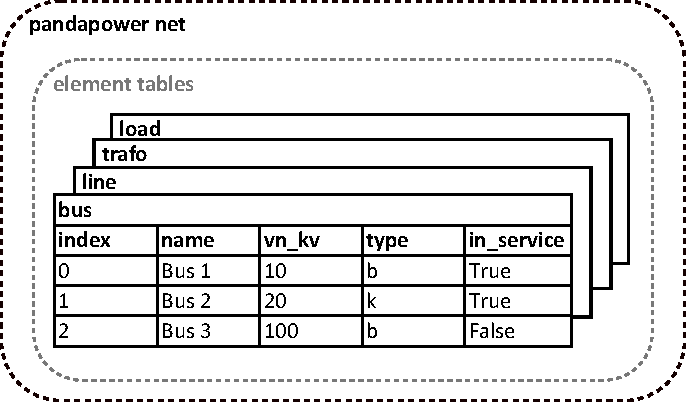
\includegraphics[width=.6\linewidth]{images/Background/Pandapower/Pandapower_net.pdf}
\caption{Pandas data frame representation of the Pandapower network}
% \label{fig:gym_anm_net}
\end{figure}


% \subsection{Network models}
% Pandapower allows to use different type of elements.

\subsection{Network models}
There are two main ways of how a power system can be defined.
A commonly used approach is the bus-branch model (BBM), which defines the network as a collection of buses which are connected by generic branches. Branches are modelled with a predefined equivalent circuit and are used to model multiple elements connected to that branch (multi-pole), like lines or transformers. Buses are attributed with power injections to model single-pole elements like loads, generators or capacitor banks. Since the BBM is an accurate mathematical representation of the network, electric equations for power systems analysis can be directly derived from it, but the need to calculate the impedances for each branch and summed power injections at each bus manually can be cumbersome and error-prone, especially for complex elements. \\
Instead of a BBM, Pandapower uses an element-based model (EBM) to model electric grids. An element is either connected to one or multiple buses and is defined with characteristic parameters. This allows defining the network parameters, such as length and relative impedance for lines, or short circuit voltage and rated apparent power for transformers. While BBM allows only the definition of a summed power injection at each bus, single-pole elements (such as load or generation elements) can be connected to buses independently. This also allows connecting multiple elements at one bus. The element models are then processed internally with the appropriate equivalent circuits to derive a mathematical description of the grid \cite{pandapower}.

\subsection{Optimal power flow}
The power flow is the most important electric analysis function for power system planning. It allows calculating the current flows and voltages in the network. \\
The Pandapower power flow solver is based on the Newton-Raphson method. The implementation is based on PYPOWER Python library. To solve the \gls{OPF}, the bus constraints include maximum and minimum voltage magnitude, active and reactive power limits can be defined for PV and slack-elements like external grids and generators, but also for PQ-elements, such as loads and static generators. \\
After defining all the network elements, to run the power flow solver it is just need to execute the command: 

\begin{algorithm}[h]
\state pandapower.runpp(net, ...)
\end{algorithm}

\noindent this function takes as input the Pandapower network data structure and some other optional values (for example the algorithm solver, max number of iterations, tolerance and so on). \\

\noindent Internally, Pandapower solves the following optimization problem:

\begin{align*}
    \min &\sum_{i \: \in \: gen, sgen, load, external grid} P_i \cdot f(P_i) \\
        \textrm{s.t.} \\
        & \text{load flow equations} \\
        & \text{branch constraints} \\
        & \text{bus constraints} \\
        & \text{operation power flow equations}
\end{align*}

\noindent where $P_i$ is the active power of any element and $f()$ is the cost function. Few example of the possible constrains are: 
\begin{align*}
        & P_{min,i} \leq P_{g} \le P_{max,i}, \; g \in gen \\
        & Q_{min,i} \leq Q_{g} \le Q_{max,i}, \; g \in gen \\
        & V_{min,i} \leq V_{g} \le V_{max,i}, \; i \in bus
\end{align*}

\noindent It is possible to customize the cost function and choosing between a piece-wise or polynomial cost function. Detailed information about the optimization problem, cost function and network constrains are available in the Pandapower documentation \cite{pandapower2}. \\

After running the power flow calculation, new tables are added to the network data frame.
\begin{figure}[H]
\centering
    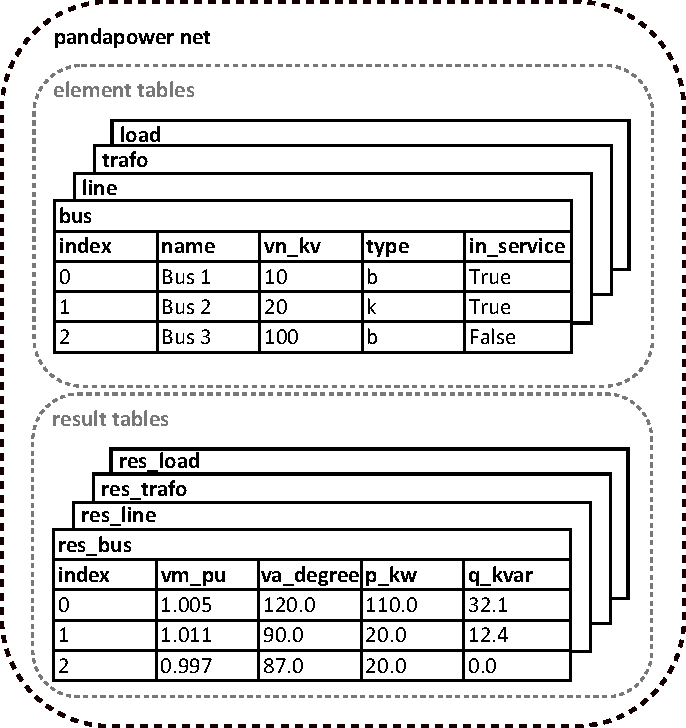
\includegraphics[width=.6\linewidth]{images/Background/Pandapower/Pandapower_resnet_big.pdf}
\caption{Pandas data frame representation of the Pandapower network after the power flow calculation}
% \label{fig:gym_anm_net}
\end{figure}

\subsection{Time series}
Pandapower allow running time series analysis for a given network. There are two main requirements for time series calculations:
\begin{itemize}
    \item a Pandapower network
    \item some time series (in a pandas data frame for example)
\end{itemize}

To execute the time series calculation, the loads, generators and other elements' active and reactive power time series have to be passed to a controller that will be in charge to change the elements' values according to the time series. \\

The time series calculation can be run with the command: 
\begin{algorithm}[h]
\state pandapower.timeseries.run\_time\_series.run\_timeseries(net, ...)
\end{algorithm}

\noindent this command will start a loop that iterates over every \textbf{time\_step}. For each step, a control loop is started for each controller by \textbf{run\_control}. The controller updates the elements' values at each step with the values given in the time series.

\begin{figure}[H]
\centering
    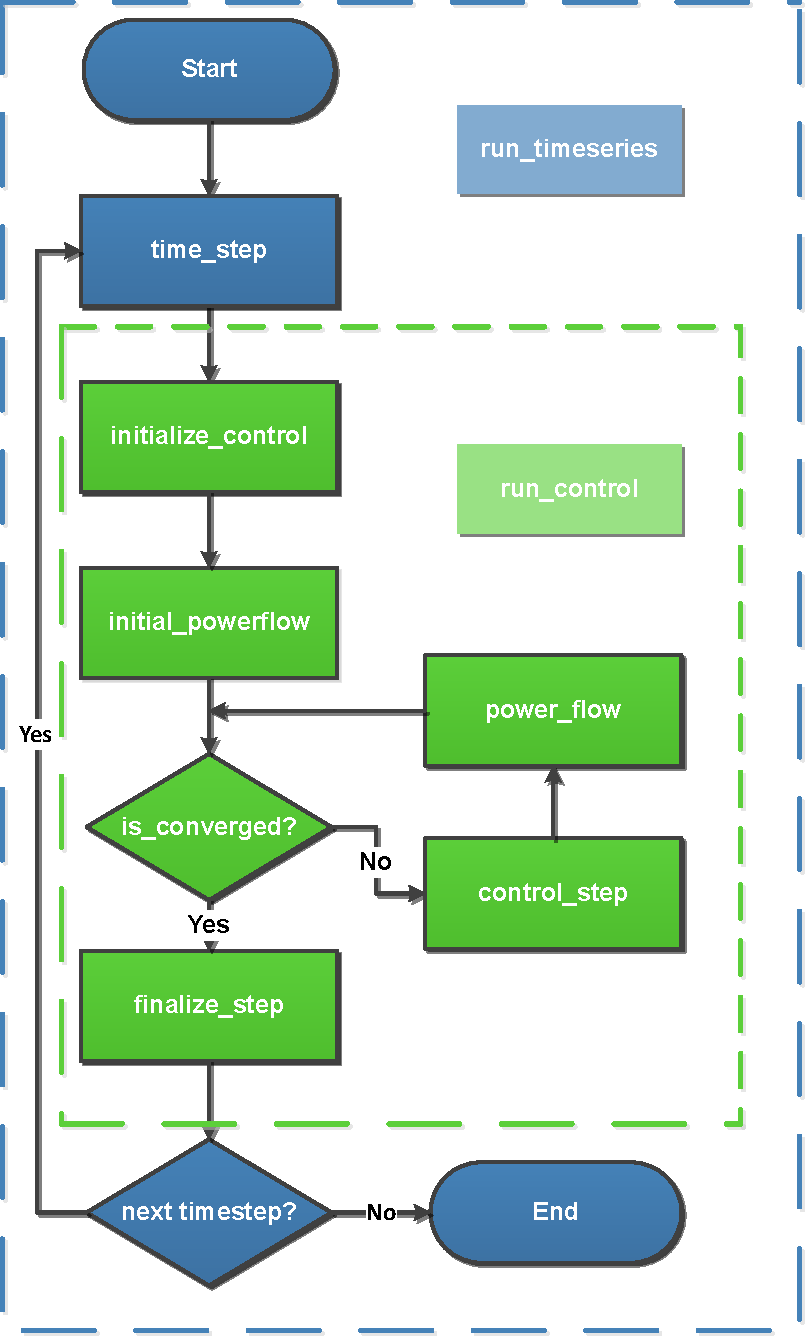
\includegraphics[width=.4\linewidth]{images/Background/Pandapower/run_timeseries_loop.pdf}
\caption{Pandapower time series calculation loop \cite{pandapowerts}}
% \label{fig:gym_anm_net}
\end{figure}

After each step, the elements' values are stored in an output writer object and this allows, after the full calculation is finished, to easily save the values on disk.

\subsection{Other functionality}
Pandapower has some other features:
\begin{itemize}
    \item Predefined Networks. In addition to creating custom networks through the application programming interface (\gls{API}), 66 predefined, published test and benchmark networks can be directly accessed through Pandapower. One of these networks, MV Oberrhein, is the one used in this thesis.
    \item Plotting features. Pandapower comes with extensive plotting features using the Matplotlib library. All Pandapower elements can be translated into different Matplotlib collections that can be customized with respect to shape, size and colour to allow highlighting and create individual network plots. It is also possible to use colour maps to codify information, like the loading of lines or the voltage at buses.
    \item Converter. Pandapower includes converters in order to export a Pandapower grid as a MATPOWER or PYPOWER casefile or the other way.
\end{itemize}